%!TEX root = ../Thesis.tex
\chapter{Stochastic Model}

\section{Stochastic System}
\label{sec:stochastic_system}

A stochastic discrete-time linear system can be written as

\begin{align}
    x_{k+1} &= Ax_k + Bu_k + w_k
    \label{eq:stochastic_state}\\
    y_k &= Cx_k + v_k
    \label{eq:stochastic_output}
\end{align}

where \(w_k\) represents the process noise and \(v_k\) represents the measurement noise. The noise terms are assumed to be zero-mean Gaussian random variables,

\begin{align}
    w_k &\sim \mathcal{N}(0,R_w)\\
    v_k &\sim \mathcal{N}(0,R_v)
\end{align}

and the initial state is assumed to be Gaussian distributed as

\begin{equation}
    x_0 \sim \mathcal{N}(\mu_0,P_0)
\end{equation}

Under these assumptions, the state distribution at time step \(k\) is characterized by its mean and covariance:

\begin{equation}
    x_k \sim \mathcal{N}(\mu_k,P_k)
\end{equation}

\subsection{State Mean}

The mean of the state is defined as

\begin{equation}
    \mu_k = \mathbb{E}[x_k]
\end{equation}

Taking the expectation of the state equation gives

\begin{align}
    \mu_{k+1}
    &=
    \mathbb{E}[x_{k+1}] \\
    &=
    \mathbb{E}[Ax_k+Bu_k+w_k]
\end{align}

Using the linearity of expectation,

\begin{equation}
    \mu_{k+1}
    =
    A\mathbb{E}[x_k]
    +
    B\mathbb{E}[u_k]
    +
    \mathbb{E}[w_k]
\end{equation}

Assuming that the control input \(u_k\) is deterministic and using

\begin{equation}
    \mathbb{E}[w_k]=0
\end{equation}

the state mean evolves according to

\begin{equation}
    \boxed{
    \mu_{k+1}
    =
    A\mu_k + Bu_k
    }
    \label{eq:state_mean}
\end{equation}

Therefore, the control input shifts the mean of the state distribution.

\subsection{State Covariance}

The state covariance is defined as

\begin{equation}
    P_k
    =
    \mathbb{E}
    \left[
        (x_k-\mu_k)
        (x_k-\mu_k)^T
    \right]
\end{equation}

From \cref{eq:stochastic_state} and \cref{eq:state_mean},

\begin{align}
    x_{k+1}-\mu_{k+1}
    &=
    Ax_k+Bu_k+w_k
    -
    \left(
        A\mu_k+Bu_k
    \right) \\
    &=
    A(x_k-\mu_k)+w_k
\end{align}

Hence,

\begin{align}
    P_{k+1}
    &=
    \mathbb{E}
    \left[
        (x_{k+1}-\mu_{k+1})
        (x_{k+1}-\mu_{k+1})^T
    \right] \\
    &=
    \mathbb{E}
    \left[
        \left(
            A(x_k-\mu_k)+w_k
        \right)
        \left(
            A(x_k-\mu_k)+w_k
        \right)^T
    \right]
\end{align}

Expanding the product gives

\begin{align}
    P_{k+1}
    &=
    A
    \mathbb{E}
    \left[
        (x_k-\mu_k)
        (x_k-\mu_k)^T
    \right]
    A^T
    \nonumber\\
    &\quad+
    \mathbb{E}[w_kw_k^T]
    \nonumber\\
    &\quad+
    A
    \mathbb{E}
    \left[
        (x_k-\mu_k)w_k^T
    \right]
    \nonumber\\
    &\quad+
    \mathbb{E}
    \left[
        w_k(x_k-\mu_k)^T
    \right]
    A^T
\end{align}

Assuming that the process noise \(w_k\) is independent of the state deviation \(x_k-\mu_k\), the cross terms are zero. Since

\begin{equation}
    \mathbb{E}[w_kw_k^T]=R_w
\end{equation}

the covariance recursion becomes

\begin{equation}
    \boxed{
    P_{k+1}
    =
    AP_kA^T+R_w
    }
    \label{eq:state_covariance}
\end{equation}

Thus, the state uncertainty propagates through the system dynamics and increases due to the process noise.

\subsection{Output Mean}

The stochastic output equation is

\begin{equation}
    y_k=Cx_k+v_k
\end{equation}

The mean of the output is therefore

\begin{align}
    \mu_{y,k}
    &=
    \mathbb{E}[y_k] \\
    &=
    \mathbb{E}[Cx_k+v_k]
\end{align}

Using the linearity of expectation and

\begin{equation}
    \mathbb{E}[v_k]=0
\end{equation}

we obtain

\begin{equation}
    \boxed{
    \mu_{y,k}
    =
    C\mu_k
    }
    \label{eq:output_mean}
\end{equation}

\subsection{Output Covariance}

The output covariance is defined as

\begin{equation}
    P_{y,k}
    =
    \mathbb{E}
    \left[
        (y_k-\mu_{y,k})
        (y_k-\mu_{y,k})^T
    \right]
\end{equation}

Using

\begin{equation}
    x_k=\mu_k+e_k
\end{equation}

where

\begin{equation}
    e_k=x_k-\mu_k
    \qquad
    \mathbb{E}[e_k]=0
\end{equation}

the output can be expressed as

\begin{align}
    y_k
    &=
    C(\mu_k+e_k)+v_k \\
    &=
    C\mu_k+Ce_k+v_k
\end{align}

Since

\begin{equation}
    \mu_{y,k}=C\mu_k
\end{equation}

the output deviation from its mean is

\begin{equation}
    y_k-\mu_{y,k}
    =
    Ce_k+v_k
\end{equation}

Therefore,

\begin{align}
    P_{y,k}
    &=
    \mathbb{E}
    \left[
        (Ce_k+v_k)
        (Ce_k+v_k)^T
    \right]
\end{align}

Expanding the expression gives

\begin{align}
    P_{y,k}
    &=
    C
    \mathbb{E}[e_ke_k^T]
    C^T
    +
    \mathbb{E}[v_kv_k^T]
    \nonumber\\
    &\quad+
    C\mathbb{E}[e_kv_k^T]
    +
    \mathbb{E}[v_ke_k^T]C^T
\end{align}

Assuming that the measurement noise \(v_k\) is independent of the state error \(e_k\), the cross terms vanish. Since

\begin{equation}
    \mathbb{E}[e_ke_k^T]=P_k
\end{equation}

and

\begin{equation}
    \mathbb{E}[v_kv_k^T]=R_v,
\end{equation}

the output covariance becomes

\begin{equation}
    \boxed{
    P_{y,k}
    =
    CP_kC^T+R_v
    }
    \label{eq:output_covariance}
\end{equation}

Therefore, the stochastic state and output distributions are completely characterized by the following recursive equations:

\begin{align}
    \mu_{k+1} &= A\mu_k+Bu_k,\\
    P_{k+1} &= AP_kA^T+R_w,\\
    \mu_{y,k} &= C\mu_k,\\
    P_{y,k} &= CP_kC^T+R_v
\end{align}

Hence,

\begin{equation}
    x_k \sim \mathcal{N}(\mu_k,P_k)
\end{equation}

while the corresponding output distribution is

\begin{equation}
    y_k
    \sim
    \mathcal{N}
    \left(
        \mu_{y,k},
        P_{y,k}
    \right)
\end{equation}

\section{Model with Chance Constraints}
\label{sec:stochastic_chance_constraints}

In stochastic systems, the output cannot in general be guaranteed to remain inside deterministic bounds at every time step because of the presence of uncertainty. Instead, the constraints can be imposed probabilistically using chance constraints.

For each prediction step \(k\), the output is required to satisfy

\begin{equation}
    \mathbb{P}
    \left(
        y_{\min}
        \leq
        y_k
        \leq
        y_{\max}
    \right)
    \geq
    1-\alpha,
    \qquad
    k=1,\ldots,N
    \label{eq:chance_constraint}
\end{equation}

where \(\alpha\) denotes the allowed probability of constraint violation.

The total violation probability is divided between the upper and lower bounds according to

\begin{equation}
    \alpha_{\mathrm{upper}}
    +
    \alpha_{\mathrm{lower}}
    =
    \alpha
    \label{eq:alpha_split}
\end{equation}

The two-sided chance constraint can therefore be handled through separate upper and lower probabilistic constraints.

\subsection*{Upper Chance Constraint}

The upper output constraint is

\begin{equation}
    \mathbb{P}
    \left(
        y_k
        \leq
        y_{\max}
    \right)
    \geq
    1-\alpha_{\mathrm{upper}}
    \label{eq:upper_chance}
\end{equation}

Since

\begin{equation}
    y_k
    \sim
    \mathcal{N}
    \left(
        \mu_{y,k},
        \sigma_{y,k}^2
    \right)
\end{equation}

the output can be standardized as

\begin{equation}
    Z
    =
    \frac{
        y_k-\mu_{y,k}
    }{
        \sigma_{y,k}
    },
    \qquad
    Z\sim\mathcal{N}(0,1)
\end{equation}

Therefore,

\begin{align}
    \mathbb{P}
    \left(
        y_k\leq y_{\max}
    \right)
    &=
    \mathbb{P}
    \left(
        Z
        \leq
        \frac{
            y_{\max}-\mu_{y,k}
        }{
            \sigma_{y,k}
        }
    \right)
\end{align}

Using the cumulative distribution function \(\Phi(\cdot)\) of the standard normal distribution,

\begin{equation}
    \Phi
    \left(
        \frac{
            y_{\max}-\mu_{y,k}
        }{
            \sigma_{y,k}
        }
    \right)
    \geq
    1-\alpha_{\mathrm{upper}}
\end{equation}

Applying the inverse standard normal cumulative distribution function yields

\begin{equation}
    \frac{
        y_{\max}-\mu_{y,k}
    }{
        \sigma_{y,k}
    }
    \geq
    \Phi^{-1}
    \left(
        1-\alpha_{\mathrm{upper}}
    \right)
\end{equation}

Rearranging gives

\begin{equation}
    \mu_{y,k}
    \leq
    y_{\max}
    -
    \Phi^{-1}
    \left(
        1-\alpha_{\mathrm{upper}}
    \right)
    \sigma_{y,k}
    \label{eq:upper_deterministic}
\end{equation}

\subsection*{Lower Chance Constraint}

Similarly, the lower output constraint is

\begin{equation}
    \mathbb{P}
    \left(
        y_k
        \geq
        y_{\min}
    \right)
    \geq
    1-\alpha_{\mathrm{lower}}
    \label{eq:lower_chance}
\end{equation}

Following the same standardization procedure gives

\begin{equation}
    \mu_{y,k}
    \geq
    y_{\min}
    +
    \Phi^{-1}
    \left(
        1-\alpha_{\mathrm{lower}}
    \right)
    \sigma_{y,k}
    \label{eq:lower_deterministic}
\end{equation}

\subsection*{Reformulation}
From the stochastic output model,

\begin{equation}
    \mu_{y,k}
    =
    C\mu_k
\end{equation}

and

\begin{equation}
    P_{y,k}
    =
    CP_kC^T+R_v
\end{equation}

For a scalar output, the standard deviation is therefore

\begin{equation}
    \sigma_{y,k}
    =
    \sqrt{
        CP_kC^T+R_v
    }
    \label{eq:output_std}
\end{equation}

Substituting these expressions into the deterministic chance constraints gives

\begin{equation}
    C\mu_k
    \leq
    y_{\max}
    -
    \Phi^{-1}
    \left(
        1-\alpha_{\mathrm{upper}}
    \right)
    \sqrt{
        CP_kC^T+R_v
    }
    \label{eq:upper_tightened}
\end{equation}

and

\begin{equation}
    C\mu_k
    \geq
    y_{\min}
    +
    \Phi^{-1}
    \left(
        1-\alpha_{\mathrm{lower}}
    \right)
    \sqrt{
        CP_kC^T+R_v
    }
    \label{eq:lower_tightened}
\end{equation}

The resulting deterministic limits are referred to as the \emph{tight bounds}. They are defined as

\begin{equation}
    \boxed{
    \tilde{y}_{\min,k}
    =
    y_{\min}
    +
    \Phi^{-1}
    \left(
        1-\alpha_{\mathrm{lower}}
    \right)
    \sigma_{y,k}
    }
    \label{eq:tight_lower_bound}
\end{equation}

and

\begin{equation}
    \boxed{
    \tilde{y}_{\max,k}
    =
    y_{\max}
    -
    \Phi^{-1}
    \left(
        1-\alpha_{\mathrm{upper}}
    \right)
    \sigma_{y,k}
    }
    \label{eq:tight_upper_bound}
\end{equation}

Hence, the original probabilistic constraint can be enforced through the deterministic condition

\begin{equation}
    \boxed{
    \tilde{y}_{\min,k}
    \leq
    C\mu_k
    \leq
    \tilde{y}_{\max,k}
    }
    \label{eq:tight_bounds}
\end{equation}

The tight bounds shrink the original feasible output interval in order to account for stochastic uncertainty. The amount of tightening depends on the output standard deviation \(\sigma_{y,k}\) and on the selected violation probabilities.

A larger uncertainty results in a larger distance between the original bounds and the tight bounds. Similarly, selecting a smaller violation probability increases that difference.
\section{Stacked Forms Derivation}
\label{sec:stochastic_stacked}

For optimization over a finite prediction horizon, the state means, output means, and control inputs are collected into stacked vectors. This allows the stochastic control problem to be expressed in a compact matrix form.

\subsection{Stacked Prediction Matrices}

The mean-state dynamics are given by

\begin{equation}
    \mu_{k+1}
    =
    A\mu_k+Bu_k
\end{equation}

Starting from the initial mean \(\mu_0\), the first predicted mean is

\begin{equation}
    \mu_1
    =
    A\mu_0+Bu_0
\end{equation}

The second predicted mean is

\begin{align}
    \mu_2
    &=
    A\mu_1+Bu_1 \\
    &=
    A(A\mu_0+Bu_0)+Bu_1 \\
    &=
    A^2\mu_0+ABu_0+Bu_1
\end{align}

Similarly,

\begin{equation}
    \mu_3
    =
    A^3\mu_0
    +
    A^2Bu_0
    +
    ABu_1
    +
    Bu_2
\end{equation}

The state means over a prediction horizon \(N\) are stacked as

\begin{equation}
    M
    =
    \begin{bmatrix}
        \mu_1 \\
        \mu_2 \\
        \vdots \\
        \mu_N
    \end{bmatrix}
\end{equation}

while the control inputs are collected in

\begin{equation}
    U
    =
    \begin{bmatrix}
        u_0 \\
        u_1 \\
        \vdots \\
        u_{N-1}
    \end{bmatrix}
\end{equation}

The stacked mean-state prediction can therefore be written as

\begin{equation}
    \boxed{
        M
        =
        \mathcal{A}\mu_0
        +
        \mathcal{B}U
    }
    \label{eq:stochastic_stacked_state}
\end{equation}

where

\begin{equation}
    \mathcal{A}
    =
    \begin{bmatrix}
        A \\
        A^2 \\
        \vdots \\
        A^N
    \end{bmatrix}
\end{equation}

and

\begin{equation}
    \mathcal{B}
    =
    \begin{bmatrix}
        B & 0 & \cdots & 0 \\
        AB & B & \cdots & 0 \\
        A^2B & AB & \cdots & 0 \\
        \vdots & \vdots & \ddots & \vdots \\
        A^{N-1}B & A^{N-2}B & \cdots & B
    \end{bmatrix}
\end{equation}

The output mean at each prediction step is

\begin{equation}
    \mu_{y,k}=C\mu_k
\end{equation}

The stacked output-mean vector is therefore defined as

\begin{equation}
    M_y
    =
    \begin{bmatrix}
        \mu_{y,1} \\
        \mu_{y,2} \\
        \vdots \\
        \mu_{y,N}
    \end{bmatrix}
\end{equation}

Defining the block-diagonal output matrix

\begin{equation}
    \mathcal{C}
    =
    I_N\otimes C
\end{equation}

the stacked output means satisfy

\begin{equation}
    M_y
    =
    \mathcal{C}M
\end{equation}

Substituting \cref{eq:stochastic_stacked_state} gives

\begin{equation}
    M_y
    =
    \mathcal{C}\mathcal{A}\mu_0
    +
    \mathcal{C}\mathcal{B}U
\end{equation}

Introducing

\begin{equation}
    F
    =
    \mathcal{C}\mathcal{A},
    \qquad
    G
    =
    \mathcal{C}\mathcal{B}
\end{equation}

the stacked output-mean prediction becomes

\begin{equation}
    \boxed{
        M_y
        =
        F\mu_0+GU
    }
    \label{eq:stochastic_stacked_output}
\end{equation}

\subsection{Stacked Cost Function}

For a stochastic output,

\begin{equation}
    y_k
    =
    \mu_{y,k}
    +
    e_{y,k}
\end{equation}

where

\begin{equation}
    \mathbb{E}[e_{y,k}]=0
\end{equation}

The expected quadratic tracking cost at one prediction step is

\begin{equation}
    \mathbb{E}
    \left[
        (y_k-\bar{y}_k)^T
        Q
        (y_k-\bar{y}_k)
    \right]
\end{equation}

Substituting

\begin{equation}
    y_k=\mu_{y,k}+e_{y,k}
\end{equation}

gives

\begin{align}
    &\mathbb{E}
    \left[
        (y_k-\bar{y}_k)^T
        Q
        (y_k-\bar{y}_k)
    \right]
    \nonumber\\
    &=
    (\mu_{y,k}-\bar{y}_k)^T
    Q
    (\mu_{y,k}-\bar{y}_k)
    +
    \mathbb{E}
    \left[
        e_{y,k}^T Qe_{y,k}
    \right]
\end{align}

Using the trace identity

\begin{equation}
    x^TQx
    =
    \operatorname{tr}
    \left(
        Qxx^T
    \right)
\end{equation}

the second term can be written as

\begin{align}
    \mathbb{E}
    \left[
        e_{y,k}^TQe_{y,k}
    \right]
    &=
    \operatorname{tr}
    \left(
        Q
        \mathbb{E}
        [e_{y,k}e_{y,k}^T]
    \right) \\
    &=
    \operatorname{tr}
    \left(
        QP_{y,k}
    \right)
\end{align}

Since

\begin{equation}
    P_{y,k}
    =
    CP_kC^T+R_v
\end{equation}

the expected tracking cost becomes

\begin{align}
    &\mathbb{E}
    \left[
        (y_k-\bar{y}_k)^T
        Q
        (y_k-\bar{y}_k)
    \right]
    \nonumber\\
    &=
    (\mu_{y,k}-\bar{y}_k)^T
    Q
    (\mu_{y,k}-\bar{y}_k)
    +
    \operatorname{tr}
    \left[
        Q(CP_kC^T+R_v)
    \right]
\end{align}

For the additive-noise stochastic system considered here, the covariance recursion

\begin{equation}
    P_{k+1}
    =
    AP_kA^T+R_w
\end{equation}

does not depend on the deterministic control input \(u_k\). Therefore,

\begin{equation}
    \operatorname{tr}
    \left[
        Q(CP_kC^T+R_v)
    \right]
\end{equation}

is constant with respect to the optimization variable \(U\) and can be omitted when determining the optimal control sequence.

The resulting optimization objective is therefore

\begin{equation}
    \phi_{\mathrm{opt}}
    =
    \frac{1}{2}
    \sum_{k=0}^{N-1}
    \left[
        (C\mu_{k+1}-\bar{y}_{k+1})^T
        Q
        (C\mu_{k+1}-\bar{y}_{k+1})
        +
        u_k^TRu_k
    \right]
\end{equation}

Define the stacked reference vector as

\begin{equation}
    \bar{Y}_{\mathrm{ref}}
    =
    \begin{bmatrix}
        \bar{y}_1 \\
        \bar{y}_2 \\
        \vdots \\
        \bar{y}_N
    \end{bmatrix}
\end{equation}

and let the stacked weighting matrices be

\begin{align}
    \bar{Q}
    &=
    \operatorname{blkdiag}
    \left(
        Q,\ldots,Q
    \right)\\
    \bar{R}
    &=
    \operatorname{blkdiag}
    \left(
        R,\ldots,R
    \right)
\end{align}

Using

\begin{equation}
    M_y=F\mu_0+GU
\end{equation}

the stacked cost function becomes

\begin{equation}
    \phi
    =
    \frac{1}{2}
    \left[
        (F\mu_0+GU-\bar{Y}_{\mathrm{ref}})^T
        \bar{Q}
        (F\mu_0+GU-\bar{Y}_{\mathrm{ref}})
        +
        U^T\bar{R}U
    \right]
    \label{eq:stochastic_stacked_cost}
\end{equation}


Expanding \cref{eq:stochastic_stacked_cost} gives

\begin{align}
    \phi
    &=
    \frac{1}{2}
    U^T
    \left(
        G^T\bar{Q}G+\bar{R}
    \right)
    U
    \nonumber\\
    &\quad+
    (F\mu_0-\bar{Y}_{\mathrm{ref}})^T
    \bar{Q}G\,U
    +
    \text{const}
\end{align}

Define

\begin{equation}
    H
    =
    G^T\bar{Q}G+\bar{R}
\end{equation}

and

\begin{equation}
    f
    =
    G^T
    \bar{Q}
    \left(
        F\mu_0-\bar{Y}_{\mathrm{ref}}
    \right)
\end{equation}

The cost function can then be written in standard quadratic-programming form as

\begin{equation}
    \boxed{
        \phi(U)
        =
        \frac{1}{2}U^THU
        +
        f^TU
    }
    \label{eq:stochastic_qp_cost}
\end{equation}


For the unconstrained problem, the stationary condition is

\begin{equation}
    \frac{\partial\phi}{\partial U}
    =
    HU+f
    =
    0
\end{equation}

and therefore

\begin{equation}
    U^\ast
    =
    -H^{-1}f
\end{equation}

\subsection{Stacked Chance Constraints}

From the chance-constraint derivation, the deterministic tight bounds at each prediction step are

\begin{equation}
    \tilde{y}_{\min,k}
    \leq
    \mu_{y,k}
    \leq
    \tilde{y}_{\max,k}
\end{equation}

The tight lower and upper bounds are stacked as

\begin{equation}
    \tilde{Y}_{\min}
    =
    \begin{bmatrix}
        \tilde{y}_{\min,1} \\
        \tilde{y}_{\min,2} \\
        \vdots \\
        \tilde{y}_{\min,N}
    \end{bmatrix}
\end{equation}

and

\begin{equation}
    \tilde{Y}_{\max}
    =
    \begin{bmatrix}
        \tilde{y}_{\max,1} \\
        \tilde{y}_{\max,2} \\
        \vdots \\
        \tilde{y}_{\max,N}
    \end{bmatrix}
\end{equation}

Therefore, the stacked deterministic chance constraint becomes

\begin{equation}
    \boxed{
        \tilde{Y}_{\min}
        \leq
        M_y
        \leq
        \tilde{Y}_{\max}
    }
\end{equation}

Using

\begin{equation}
    M_y
    =
    F\mu_0+GU
\end{equation}

this becomes

\begin{equation}
    \tilde{Y}_{\min}
    \leq
    F\mu_0+GU
    \leq
    \tilde{Y}_{\max}
\end{equation}

Rearranging with respect to the optimization variable \(U\) gives

\begin{equation}
    \boxed{
        \tilde{Y}_{\min}-F\mu_0
        \leq
        GU
        \leq
        \tilde{Y}_{\max}-F\mu_0
    }
    \label{eq:stochastic_stacked_constraints}
\end{equation}

\subsection*{Overview}

Combining the stacked cost function and the tight chance constraints, the stochastic optimal control problem can be written as

\begin{equation}
\boxed{
\begin{aligned}
    \min_U
    \quad &
    \frac{1}{2}U^THU+f^TU
    \\[1mm]
    \text{subject to}
    \quad &
    \tilde{Y}_{\min}-F\mu_0
    \leq
    GU
    \leq
    \tilde{Y}_{\max}-F\mu_0
\end{aligned}
}
\label{eq:stochastic_final_qp}
\end{equation}

\section{Open-Loop Implementation}
\label{sec:stochastic_open_loop}

The open-loop implementation follows the same general structure as the deterministic LTI open-loop case. The optimal input sequence is computed once at the beginning of the simulation and is not updated afterwards.

For the stochastic system, however, the resulting controller performance is evaluated using Monte Carlo simulation. A single optimal control sequence \(U^\ast\) is first obtained from the stochastic optimization problem. The same sequence is then applied to a large number of independently generated monte carlo trajectories.

The optimization problem is

\begin{equation}
\begin{aligned}
    \min_U
    \quad &
    \frac{1}{2}U^THU+f^TU
    \\
    \text{subject to}
    \quad &
    \tilde{Y}_{\min}-F\mu_0
    \leq
    GU
    \leq
    \tilde{Y}_{\max}-F\mu_0
\end{aligned}
\end{equation}

Solving this problem yields the optimal open-loop input sequence

\begin{equation}
    U^\ast
    =
    \begin{bmatrix}
        u_0^\ast \\
        u_1^\ast \\
        \vdots \\
        u_{N-1}^\ast
    \end{bmatrix}
\end{equation}

This sequence is calculated only once using the initial mean and covariance, the reference trajectory, and the tight output bounds.

The stochastic open-loop procedure can therefore be summarized as follows:

\begin{enumerate}
    \item Select \(N\), \(\mu_0\), \(P_0\), \(Q\), \(R\), \(R_w\), \(R_v\), the reference trajectory, and the chance-constraint parameters.

    \item Propagate the state covariance and construct the corresponding tight bounds
    \[
        \tilde{Y}_{\min},
        \qquad
        \tilde{Y}_{\max}
    \]

    \item Construct the stacked prediction matrices and the quadratic-programming matrices \(H\) and \(f\).

    \item Solve the stochastic open-loop optimization problem once to obtain
    \[
        U^\ast
    \]

    \item Generate \(n_{\mathrm{MC}}\) independent Monte Carlo realizations of the initial state and stochastic noise.

    \item Apply the same optimal sequence \(U^\ast\) to every Monte Carlo trajectory.

    \item Simulate all trajectories using the stochastic state and output equations.

    \item Evaluate the resulting tracking performance and the empirical constraint-satisfaction probability.
\end{enumerate}

\subsection{Results}
\label{subsec:stochastic_open_loop_results}

The stochastic open-loop controller was evaluated using a two-state linear system over a prediction horizon of

\begin{equation}
    N = 30
\end{equation}

The system matrices were selected as

\begin{equation}
    A =
    \begin{bmatrix}
        0.90 & 1.00 \\
        0.00 & 0.50
    \end{bmatrix},
    \qquad
    B =
    \begin{bmatrix}
        0.0 \\
        1.0
    \end{bmatrix}
\end{equation}

with both states directly observed at the output:

\begin{equation}
    C =
    \begin{bmatrix}
        1 & 0 \\
        0 & 1
    \end{bmatrix}
\end{equation}

The state and input weighting matrices were chosen as

\begin{equation}
    Q = I_2,
    \qquad
    R = 0.1
\end{equation}

The process and measurement noise covariance matrices were defined as

\begin{equation}
    R_w =
    \begin{bmatrix}
        0.005 & 0 \\
        0 & 0.005
    \end{bmatrix}
\end{equation}

and

\begin{equation}
    R_v =
    \begin{bmatrix}
        0.005 & 0 \\
        0 & 0.005
    \end{bmatrix}
\end{equation}

The initial state distribution was specified by

\begin{equation}
    \mu_0 =
    \begin{bmatrix}
        0 \\
        0
    \end{bmatrix}
\end{equation}

and

\begin{equation}
    P_0 =
    \begin{bmatrix}
        0.01 & 0 \\
        0 & 0.01
    \end{bmatrix}
\end{equation}

The output constraints were imposed equally on both outputs as

\begin{equation}
    y_{\min}
    =
    \begin{bmatrix}
        -1.7 \\
        -1.7
    \end{bmatrix}
    \qquad
    y_{\max}
    =
    \begin{bmatrix}
        3.5 \\
        3.5
    \end{bmatrix}
\end{equation}

The upper and lower risk allocations were selected as

\begin{equation}
    \alpha_{\mathrm{lower}} = 0.01,
    \qquad
    \alpha_{\mathrm{upper}} = 0.01
\end{equation}

These values were used to compute the corresponding tight bounds at each prediction step according to the propagated output covariance.

The reference trajectory was divided into two operating periods. During the first 15 steps, the desired output was

\begin{equation}
    \bar{y}^{(1)}
    =
    \begin{bmatrix}
        3.1 \\
        -1.3
    \end{bmatrix}
\end{equation}

while during the second 15 steps the reference was changed to

\begin{equation}
    \bar{y}^{(2)}
    =
    \begin{bmatrix}
        -1.3 \\
        3.1
    \end{bmatrix}
\end{equation}

Thus, the reference schedule is

\begin{equation}
    \bar{y}_k
    =
    \begin{cases}
        [\,3.1 \;\; -1.3\,]^T,
        & k=1,\ldots,15\\[1mm]
        [\,-1.3 \;\; 3.1\,]^T,
        & k=16,\ldots,30
    \end{cases}
\end{equation}

The control input was constrained by

\begin{equation}
    -5.0 \leq u_k \leq 5.0
\end{equation}

A single optimal open-loop input sequence \(U^\ast\) was obtained by solving the stacked stochastic optimization problem. This same sequence was then applied to all Monte Carlo trajectories.

\begin{figure}[H]
    \centering
    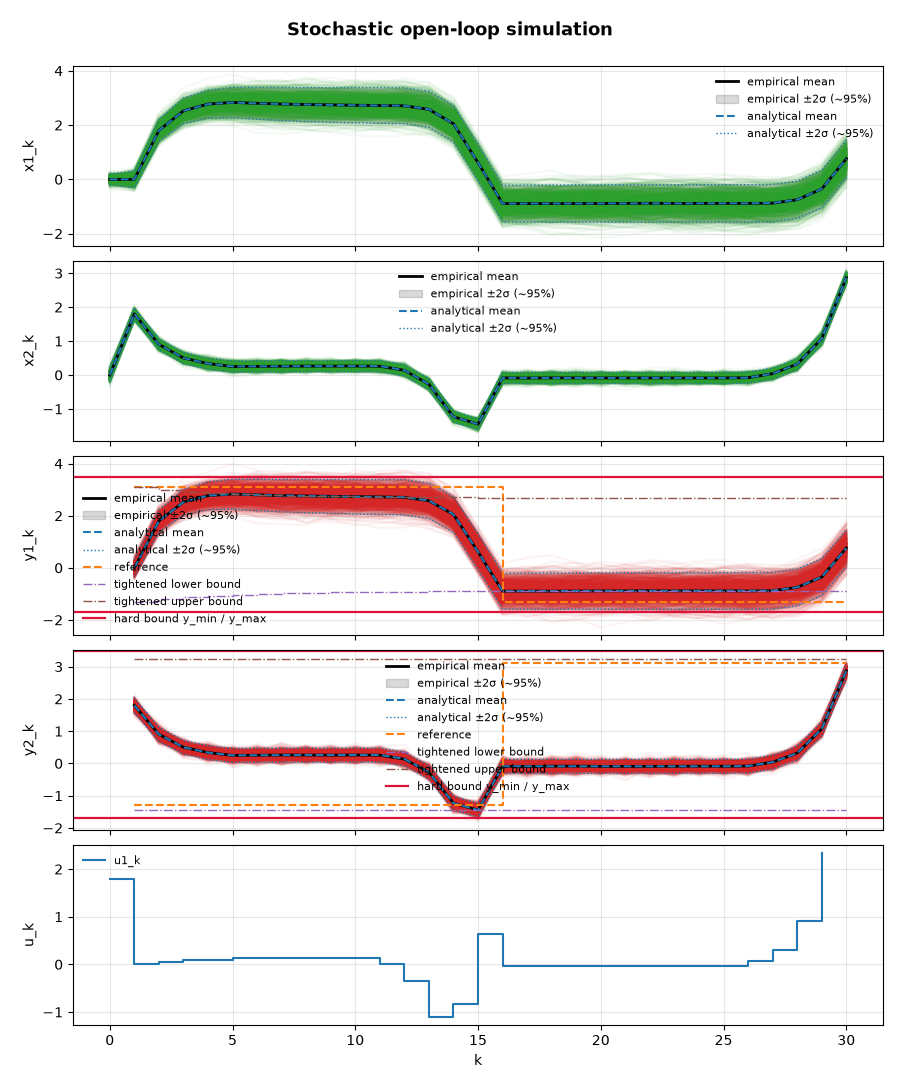
\includegraphics[width=0.9\textwidth]{graphics/stochastic_open_loop.png}
    \caption{Monte Carlo output trajectories for the stochastic open-loop implementation together with the reference trajectory, original output constraints, and tight bounds}
    \label{fig:stochastic_open_loop_outputs}
\end{figure}

\section{Closed-Loop Implementation}
\label{sec:stochastic_closed_loop}

The closed-loop stochastic implementation follows the same receding-horizon structure used in the LTI closed-loop Case. The main difference is that the controller is evaluated using Monte Carlo simulation, and each stochastic realization solves its own optimization problem using its own current state.

For each Monte Carlo trajectory \(j\), the initial state is sampled independently as

\begin{equation}
    x_0^{(j)}
    \sim
    \mathcal{N}(\mu_0,P_0)
\end{equation}

Since the realizations start from different initial conditions and are affected by independent process and measurement noise, the state of each trajectory evolves differently.

At every time step \(k\), each trajectory therefore constructs and solves its own model predictive control problem.


The stochastic closed-loop implementation can therefore be summarized as follows:

\begin{enumerate}
    \item Select \(N\), \(N_c\), \(N_{\mathrm{end}}\), \(Q\), \(R\), \(R_w\), \(R_v\), the reference trajectory, and the chance-constraint parameters.

    \item Generate \(n_{\mathrm{MC}}\) independent initial states
    \[
        x_0^{(j)}
        \sim
        \mathcal{N}(\mu_0,P_0)
    \]

    \item For each Monte Carlo trajectory \(j\), use its current state \(x_k^{(j)}\) as the initial condition of the MPC prediction.

    \item Construct the reference vector \(\bar{Y}_k\) over the current prediction horizon.

    \item Construct the corresponding tight bounds
    \[
        \tilde{Y}_{\min,k},
        \qquad
        \tilde{Y}_{\max,k}
    \]

    \item Solve a separate constrained MPC problem for each Monte Carlo realization to obtain
    \[
        U_k^{\ast,(j)}
    \]

    \item Apply only the first control action
    \[
        u_k^{(j)}
        =
        u_{k|k}^{\ast,(j)}
    \]

    \item Sample the process and measurement noise and update each stochastic trajectory independently.

    \item Shift the prediction horizon and repeat the optimization for every realization at the next time step.

    \item Continue until \(k=N_{\mathrm{end}}-1\).
\end{enumerate}

\subsection{Results}
\label{subsec:stochastic_closed_loop_results}

The closed-loop stochastic controller was evaluated using the same system, noise levels, output constraints, reference trajectory, and weighting matrices used in the open-loop experiment.



\begin{figure}[H]
    \centering
    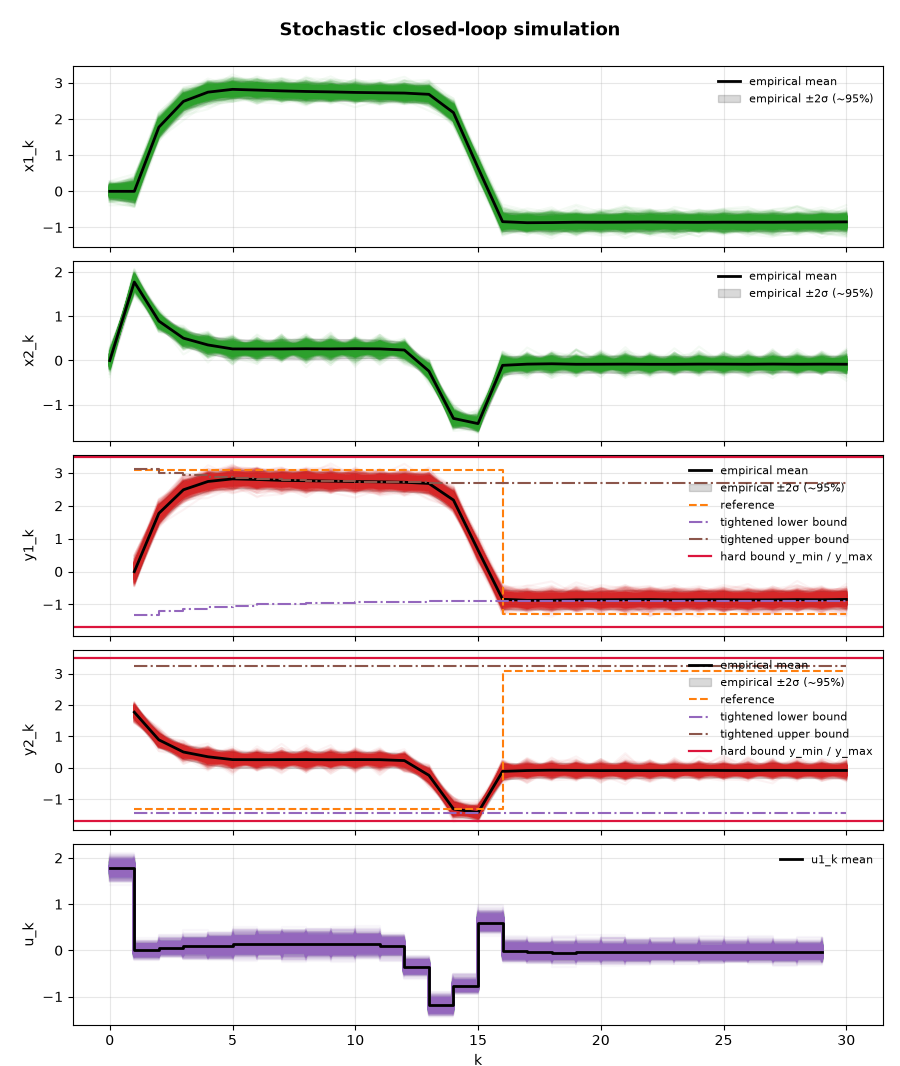
\includegraphics[width=0.9\textwidth]{graphics/stochastic_closed_loop.png}
    \caption{Monte Carlo output trajectories for the stochastic closed-loop implementation together with the reference trajectory, original output constraints, and tight bounds}
    \label{fig:stochastic_closed_loop_outputs}
\end{figure}

